
\section{Auswertung}
\label{sec:Auswertung}

\begin{table}
  \centering
  \caption{Aufgenomme Werte }
  \label{tab:werte}
  \sisetup{round-mode = places , round-precision = 2}
  \begin{tabular}{S S S S S S}
    \toprule
    {$t/\si{\minute}$} & {$T_1/\si{\celsius}$} & {$T_2/\si{\celsius}$} & {$p_A/\si{\bar}$} & {$p_B/\si{\bar}$} & {$P/\si{\watt}$} \\
    \midrule
    0         & 19.9 & 19.9 & 5    & 5.25  &  / \\
    1         & 20.6 & 19.9 & 2.4  & 6.5   &  170\\
    2         & 21.6 & 19.8 & 2.6  & 7.0     &  178\\
    3         & 22.9 & 18.9 & 3.0    & 7.25  &  185\\
    4         & 24.6 & 17.4 & 3.0    & 7.5    & 195\\
    5         & 26.5 & 15.6 & 3.2  & 8.0     &  200\\
    6         & 28.6 & 13.7 & 3.2  & 8.5     &205\\
    7         & 30.5 & 11.9 & 3.2  & 8.75   & 205\\
    8         & 32.6  &9.9  & 3.2  & 9.25   & 207\\
    9         & 34.5 & 8.0  & 3.2  & 9.5    & 210\\
    10        & 36.5 & 6.3  & 3.2  & 10.0     & 208\\
    11        & 38.4 & 4.4  & 3.2  & 10.5   & 210\\
    12        & 40   & 3.0  & 3.2  & 10.75  & 213\\
    13        & 41.7 & 1.9   &3.2  & 11.25  & 213\\
    14        & 43.3 & 1.0  & 3.2  & 11.5   & 210\\
    15        & 44.9 & 0.4  & 3.2  & 12.0     & 208\\
    16        & 46.3 & -0.2 & 3.2  & 12.25  & 205\\
    17        & 47.6 & -0.7 & 3.2  & 12.5   & 205\\
    18        & 48.7 & -1.1 & 3.2  & 12.75  & 202\\
    19        & 49.9 & -1.6 & 3.2  & 13.0     & 201\\
    20        & 50.9 & -1.9 & 3.25 & 13.5   & 200\\
    \bottomrule
  \end{tabular}
\end{table}

\paragraph{Temperaturverläufe}
Sämtliche in diesem Versuch aufgenommenen Werte lassen sich Tabelle \ref{tab:werte} entnehmen. Die Temperaturverläufe sind des Weiteren in Abb. \ref{fig:temp} dargestellt, wobei als Fit-Funktion
\begin{equation}
  T(t) = \frac{At^\alpha}{1+Bt^\alpha} +C
\end{equation}
gewählt wird und $T_2$ lediglich bis Minute $15$ gefittet wird, da anschließend der Temperaturverlauf durch Eisbildung beeinflusst wird.

\begin{figure}
  \centering
  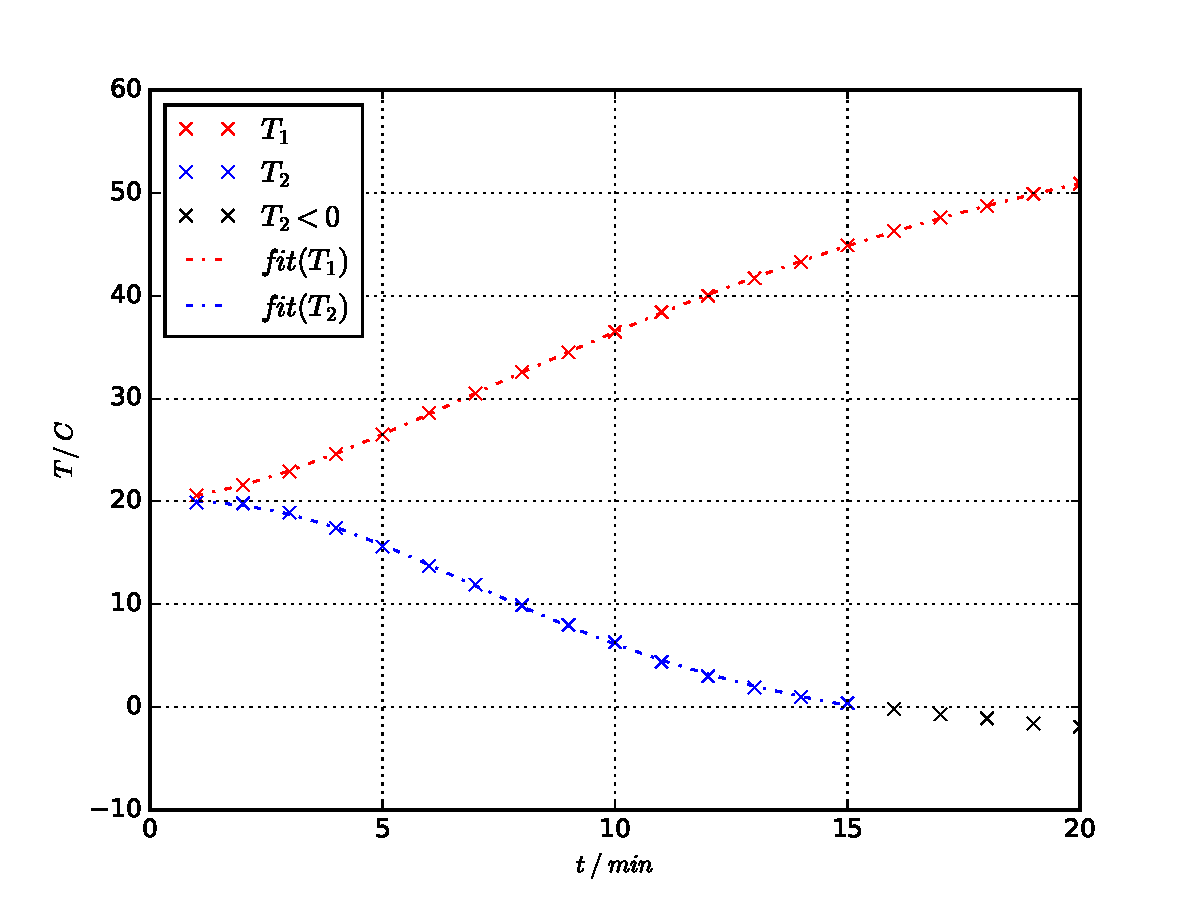
\includegraphics[width = \textwidth]{./Plots/Temperaturverlauf.pdf}
  \caption{Verlauf der Temperaturen $T_1$ und $T_2$ sowie Fits.}
  \label{fig:temp}
\end{figure}

Die Fit-Parameter für $T_1$ ergeben sich so zu:
\begin{align*}
  A_1 &= (0.454 \pm 0.020) \si{\celsius} \si{\minute}^{-1.73} \\
  B_1 &= (9.11 \pm 0.28)\cdot 10^{-3} \si{\minute}^{1.73} \\
  C_1 &= (20.12 \pm 0.07) \si{\celsius} \\
  \alpha_1 & = -1.73 \pm 0.02
\end{align*}
Für $T_2$ gilt entsprechend:
\begin{align*}
  A_2 &= (-0.255 \pm 0.095) \si{\celsius} \si{\minute}^{-2} \\
  B_2 &= (7.75 \pm 2.1) \si{\minute}^{-2} \\
  C_2 &= (20.77 \pm 0.35) \si{\celsius} \\
  \alpha_2 & = 2.00 \pm 0.19
\end{align*}

$\frac{\symup{dT}}{\symup{dt}}$ ist durch
\begin{equation}
  \frac{\symup{dT}}{\symup{dt}} = \frac{\alpha At^{\alpha-1}}{\left(1+Bt^\alpha \right)^2}
\end{equation}
gegeben.

Hierraus ergeben sich die folgenden Differentialquotienten:
\begin{align*}
  \frac{\symup{dT_1}}{\symup{dt}}(4) &= (1.8 \pm 0.6) \si{\celsius \per \minute} \\
  \frac{\symup{dT_1}}{\symup{dt}}(8) &= (2.0 \pm 0.7) \si{\celsius \per \minute}\\
  \frac{\symup{dT_1}}{\symup{dt}}(12) &= (1.7\pm 0.4) \si{\celsius \per \minute}\\
  \frac{\symup{dT_1}}{\symup{dt}}(15) &= (1.44 \pm 0.19)\si{\celsius \per \minute}
\end{align*}
bzw.
\begin{align*}
  \frac{\symup{dT_2}}{\symup{dt}}(4) &= (-1.6 \pm 0.8) \si{\celsius \per \minute} \\
  \frac{\symup{dT_2}}{\symup{dt}}(8) &= (-1.8 \pm 0.9) \si{\celsius \per \minute}\\
  \frac{\symup{dT_2}}{\symup{dt}}(12)&= (-1.4\pm 0.6)  \si{\celsius \per \minute}\\
  \frac{\symup{dT_2}}{\symup{dt}}(15)&= (-1.0\pm 0.5) \si{\celsius \per \minute}
\end{align*}

\paragraph{Güte der Apparatur}

Es lässt sich nun aus diesen Werten die Güte $\nu$ über \eqref{eqn:q1} bzw. \eqref{eqn:q2} und \eqref{eqn:realGüte} mitteln. Hierbei wird die Wärmekapazität $c_w \approx 4.2 \si{\kilo \joule \per \kilo \gram \celsius}$ \cite{Stoffwerte} angenommen. Die Masse des Wasser beträgt $m_1 m_2 = 3 \si{\kilo \gram}$, die Wärmekapazität der Kupferleitungen beträgt $m_k c_k = 0.66 \si{\kilo \joule \per \kilo \gram \celsius}$.
Diese Werte liefern die in Tabelle \ref{tab:nu} hinterlegten Güteziffern.

\begin{table}
  \centering
  \caption{Güteziffern $\nu$, zum Zeitpunkt $t$.}
  \label{tab:nu}
  \sisetup{round-mode = places , round-precision = 2}
  \begin{tabular}{S S S}
    \toprule
    {$t/\si{\minute}$} & {$\nu$} & {$\nu_{ideal}$}\\
    \midrule
    4   & {$0.12 \pm 0.04$} & 3.42\\
    8   & {$0.13 \pm 0.04$} & 1.44\\
    12  & {$0.11 \pm 0.03$} & 1.08\\
    15  & {$0.09 \pm 0.01$} & 1.01\\
    \bottomrule
  \end{tabular}
\end{table}

\paragraph{Massendurchsatz}

\begin{figure}
  \centering
  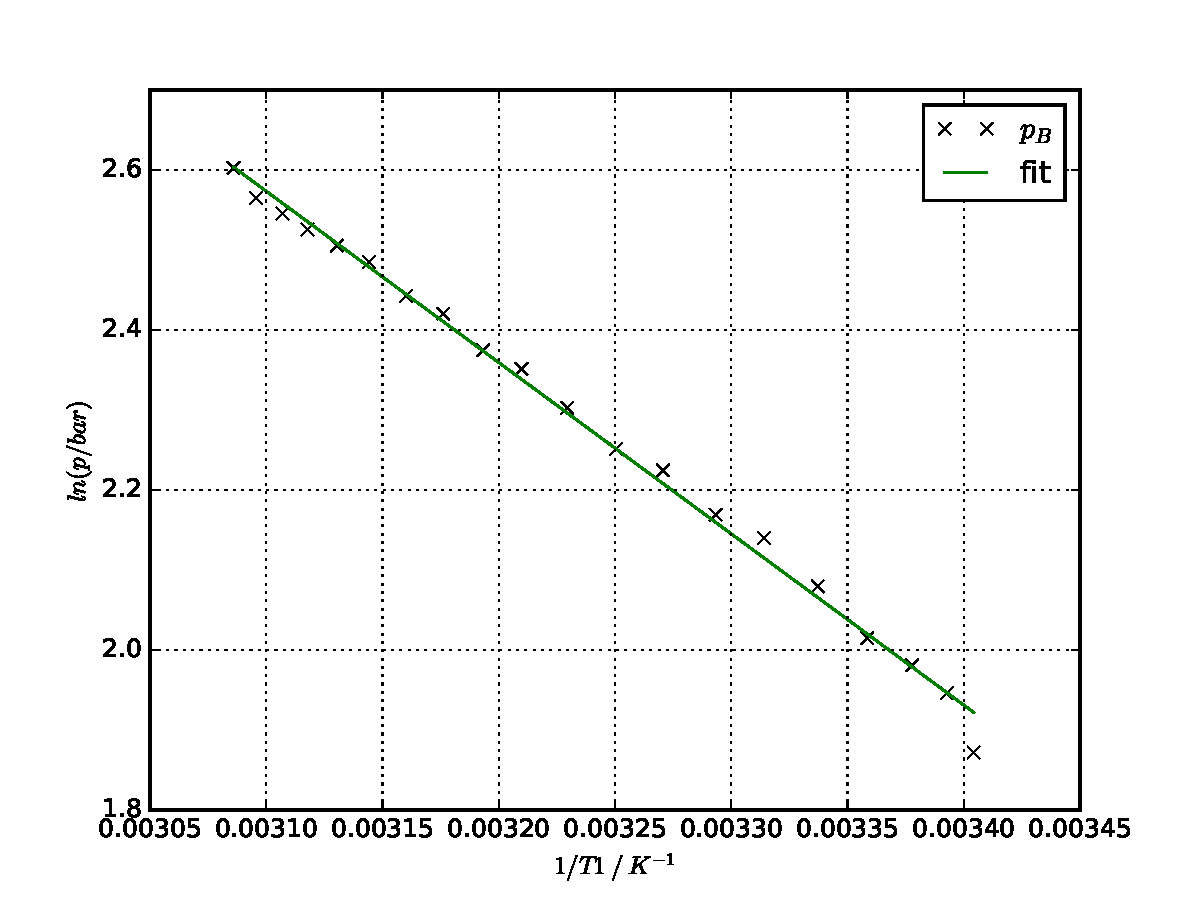
\includegraphics[width = \textwidth]{./Plots/Druck.pdf}
  \caption{Logarithmus des Gasdrucks in Abhängigkeit der reziprogen Temperatur}
  \label{fig:druck}
\end{figure}

Zur Bestimmung des Massendurchsatzes wird zunächst die Verdampfungswärme $L$ aus den aufgenommenen Daten für den Druck ermittelt. Hierzu wird in Abb. \ref{druck} zunächst der Logarithmus des Druckes $p_b$ gegen $1/T1$ aufgetragen und ein linearer Fit der Form $f(x) = a*x+b$ furchgeführt. Bei gegebenen Werten erhält man $a = -(2141 \pm 35) \si{\kelvin}$ und $b = 9.21 \pm 0.12)$. Aus dem Zusammenhang $a = -L/R$ erhält man mit der allgemeinen Gaskonstante $R = (8.31)\si{\joule \per \kelvin \mol} $ \cite{Gaskonstante} $L=(17.79 \pm 0.29) \si{\kilo \joule \per \mol}$ Die molare Masse des verwendeten Dichlordiflourmethan beträgt $m_{mol} = 0.120913 \si{\kilo \gram \per \mol}$ \cite{Gas}, folglich erhält man
\begin{equation}
  L=(147\pm 2) \si{\kilo \joule \per \kilo \gram}.
  \label{eqn:L}
\end{equation}
Es ergibt sich somit der Massendurchsatz über
\begin{equation}
  \frac{\symup{d}m}{\symup{d}t} = \frac{1}{L}(m_2 c_w + m_k c_k) \frac{\symup{d}T_2}{\symup{d}t}
\end{equation}
zu den in Tabelle \ref{tab:dm} dargestellten Werten.

\begin{table}
  \centering
  \caption{Güteziffern $\nu$, zum Zeitpunkt $t$.}
  \label{tab:dm}
  \sisetup{round-mode = places , round-precision = 2}
  \begin{tabular}{S S}
    \toprule
    {$t/\si{\minute}$} & {$\frac{\symup{d}m}{\symup{d}t}/\si{\kilo \gram \per \minute}$}\\
    \midrule
    4   & {$0.14 \pm 0.07$} \\
    8   & {$0.16 \pm 0.08$} \\
    12  & {$0.13 \pm 0.05$} \\
    15  & {$0.09  \pm 0.05$} \\
    \bottomrule
  \end{tabular}
\end{table}

\paragraph{Kompressorleistung}
Für das hier verwendete Dichlordifluormethan gilt: $\rho_0 =5.51 \, \symup{kg m^3}$ und $\kappa = 1.14$. Über die ideale Gasgleichung ergibt sich $\rho = \frac{\rho_0 p_a T_0}{p_0 T_2}$.
So erhält man:
\begin{align*}
N(4min) &= (1.0 \pm 0.5) \cdot 10^2 \si{\watt} \\
N(8min) &=  (1.3 \pm 0.6)\cdot 10^2 \si{\watt} \\
N(12min) &=  (1.1 \pm 0.5)\cdot 10^2 \si{\watt} \\
N(15min) &=  (9 \pm 4)\cdot 10^1 \si{\watt}
\end{align*}
